
The verification of execution relies on a concept called
zero-knowledge proof. A zero-knowledge proof is a cryptographic
protocol that is one party, the prover, to prove to another party that
some statement is true without revealing additional information.

The verifier takes as input the ciphertexts, the output messages and
the extra data, the zero-knowledge proofs, created by each mix
server. It then performs a series of calculations determining whether
the mix-net was executed correctly or not and outputs this result.

\vspace{14pt}

\begin{center}
  \makebox[\textwidth]{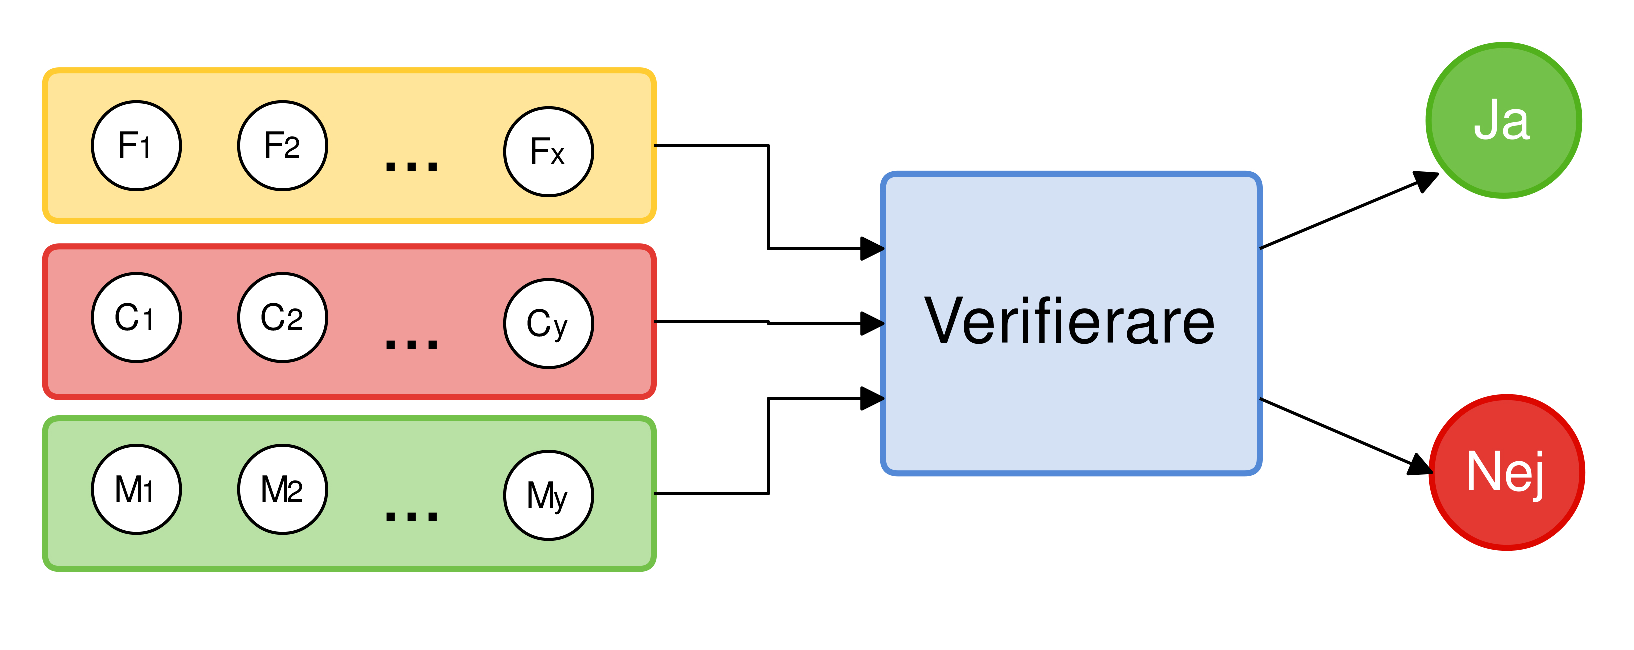
\includegraphics[width=\textwidth]{../presentation/images/mix3.pdf}}
\end{center}

